\begin{frame}
	\only<1-2>
	{
		\begin{columns}
			\begin{column}{0.7\textwidth}
				\centering
				\begin{exampleblock}{Exemplo 1 - Modelo Matemático Completo}
					\scriptsize
					\begin{table}
						\begin{tabular}{r c l}
							$ \max Z = 600x_1+800x_2$ & 
\includegraphics[width=0.8cm,height=0.2cm]{seta2.png} & Função Objetivo \\
							sujeito a & & \\
							$x_1+x_2 \le 100$ & 
\includegraphics[width=0.8cm,height=0.2cm]{seta2.png}& Área Cultivo \\
							$3x_1+2x_2 \le 240$ & 
\includegraphics[width=0.8cm,height=0.2cm]{seta2.png}& Mão de Obra \\
							$x_1 \le 60 $ & 
\includegraphics[width=0.8cm,height=0.2cm]{seta2.png}& Produção Cereal \textbf{A} \\
							$x_2 \le 80 $ &
\includegraphics[width=0.8cm,height=0.2cm]{seta2.png} & Produção Cereal \textbf{B} \\
							$x_1, x_2 \ge 0$ & 
\includegraphics[width=0.8cm,height=0.2cm]{seta2.png}& Produção \\
						\end{tabular}
					\end{table}
				\end{exampleblock}
			\end{column}
			\begin{column}{0.3\textwidth}
				\centering
				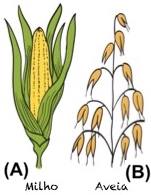
\includegraphics[width=2cm,height=3cm]{milho_aveia2.png}
			\end{column}
		\end{columns}
	}

	\only<1>
	{
		\begin{block}{Forma Padrão - {\color{cyan}Escolha 1} - Solução Básica Factível Inicial}
			\begin{columns}
				\begin{column}{0.35\textwidth}
					$
						\begin{matrix}
							\max Z - 600x_1 - 800x_2 = 0 \\
						\end{matrix}
					$ \\
					\text{Sujeito a:} \\
					$
						\begin{matrix}
							x_1+x_2  {+\color{red}x_3} = 100 \\
							3x_1+2x_2 {+ \color{red}x_4} = 240 \\
							x_1  {+ \color{red}x_5} = 60 \\
							x_2 {+ \color{red}x_6} = 80 \\
							x_1,x_2, {\color{red} x_3, x_4, x_5, x_6} \ge 0 \\
						\end{matrix}
					$
				\end{column}
				\vline
				\hspace{0.1cm}
				\begin{column}{0.45\textwidth}
					$
						\begin{matrix}
							\text{VB} \left\{  \begin{matrix}
														 x_3 = 100 \\
														 x_4 = 240 \\
														 x_5 = 60 \\
														 x_6 = 80 \\
								   \end{matrix} 
						   \right.
							&
							\text{VNB} \left\{  \begin{matrix}
														 x_1 = 0 \\
														 x_2 = 0 \\
								   \end{matrix} 
						   \right. 
							\\
							 & \\
						\end{matrix}
					$
					$ {\color{red}Z = 0} $
				\end{column}
			\end{columns}
		\end{block}
	}
	\only<2>
	{
 		\begin{block}{Tableau Simplex}
 			\begin{table}
 				\begin{tabular}{c c c c c c c c c}
					& \cellcolor{blue!80} \color{white} $ \scriptstyle z$
					& \cellcolor{blue!80} \color{white} $ \scriptstyle x_1$ 
					& \cellcolor{blue!80} \color{white} $ \scriptstyle x_2$
					& \cellcolor{blue!80} \color{red} $ \scriptstyle x_3$
					& \cellcolor{blue!80} \color{red} $ \scriptstyle x_4$
					& \cellcolor{blue!80} \color{red} $ \scriptstyle x_5$
					& \cellcolor{blue!80} \color{red} $ \scriptstyle x_6$ 
					& \cellcolor{blue!80} \color{white} $ \scriptstyle b$ \\
					\cellcolor{blue!80} \color{red} $ \scriptstyle x_3$
					& \cellcolor{yellow!60}  $ \scriptstyle 0$
					& \cellcolor{yellow!60}  $ \scriptstyle 1$ 
					& \cellcolor{yellow!60}  $ \scriptstyle 1$
					& \cellcolor{yellow!60}  $ \scriptstyle 1$
					& \cellcolor{yellow!60}  $ \scriptstyle 0$
					& \cellcolor{yellow!60}  $ \scriptstyle 0$
					& \cellcolor{yellow!60}  $ \scriptstyle 0$ 
					& \cellcolor{yellow!60}  $ \scriptstyle 100$ \\ 
					\cellcolor{blue!80} \color{red} $ \scriptstyle x_4$
					& \cellcolor{yellow!60}  $ \scriptstyle 0$
					& \cellcolor{yellow!60}  $ \scriptstyle 3$ 
					& \cellcolor{yellow!60}  $ \scriptstyle 2$
					& \cellcolor{yellow!60}  $ \scriptstyle 0$
					& \cellcolor{yellow!60}  $ \scriptstyle 1$
					& \cellcolor{yellow!60}  $ \scriptstyle 0$
					& \cellcolor{yellow!60}  $ \scriptstyle 0$ 
					& \cellcolor{yellow!60}  $ \scriptstyle 240$ \\ 
					\cellcolor{blue!80} \color{red} $ \scriptstyle x_5$  
					& \cellcolor{yellow!60}  $ \scriptstyle 0$
					& \cellcolor{yellow!60}  $ \scriptstyle 1$ 
					& \cellcolor{yellow!60}  $ \scriptstyle 0$
					& \cellcolor{yellow!60}  $ \scriptstyle 0$
					& \cellcolor{yellow!60}  $ \scriptstyle 0$
					& \cellcolor{yellow!60}  $ \scriptstyle 1$
					& \cellcolor{yellow!60}  $ \scriptstyle 0$ 
					& \cellcolor{yellow!60}  $ \scriptstyle 60$ \\
					\cellcolor{blue!80} \color{red} $ \scriptstyle x_6$
					& \cellcolor{yellow!60}  $ \scriptstyle 0$
					& \cellcolor{yellow!60}  $ \scriptstyle 0$ 
					& \cellcolor{yellow!60}  $ \scriptstyle 1$
					& \cellcolor{yellow!60}  $ \scriptstyle 0$
					& \cellcolor{yellow!60}  $ \scriptstyle 0$
					& \cellcolor{yellow!60}  $ \scriptstyle 0$
					& \cellcolor{yellow!60}  $ \scriptstyle 1$ 
					& \cellcolor{yellow!60}  $ \scriptstyle 80$ \\
					\cellcolor{blue!80} \color{white} $ \scriptstyle z$
					& \cellcolor{yellow!60}  $ \scriptstyle 1$
					& \cellcolor{yellow!60}  $ \scriptstyle -600$ 
					& \cellcolor{yellow!60}  $ \scriptstyle -800$
					& \cellcolor{yellow!60}  $ \scriptstyle 0$
					& \cellcolor{yellow!60}  $ \scriptstyle 0$
					& \cellcolor{yellow!60}  $ \scriptstyle 0$
					& \cellcolor{yellow!60}  $ \scriptstyle 0$ 
					& \cellcolor{yellow!60}  $ \scriptstyle 0$ \\
 				\end{tabular}
 			\end{table}
 		\end{block}
 	}
\end{frame}

\begin{frame}
	\only<1-4>
	{
	\frametitle{Tableau Simplex - {\color{cyan} Iteração 1}} 
	}
	\only<5-8>
	{
	\frametitle{Tableau Simplex - {\color{cyan} Iteração 2}} 
	}
	\only<9->
	{
	\frametitle{Tableau Simplex - {\color{cyan} Iteração 3}} 
	}

	\only<1>
	{
		\begin{table}
			\begin{tabular}{c c c c c c c c c c c c}
				& \cellcolor{blue!80} \color{white} $ \scriptstyle z$
				& \cellcolor{blue!80} \color{white} $ \scriptstyle x_1$ 
				& \cellcolor{blue!80} \color{white} $ \scriptstyle x_2$
				& \cellcolor{blue!80} \color{red} $ \scriptstyle x_3$
				& \cellcolor{blue!80} \color{red} $ \scriptstyle x_4$
				& \cellcolor{blue!80} \color{red} $ \scriptstyle x_5$
				& \cellcolor{blue!80} \color{red} $ \scriptstyle x_6$ 
				& \cellcolor{blue!80} \color{white} $ \scriptstyle b$ \\
				\cellcolor{blue!80} \color{red} $ \scriptstyle x_3$
				& \cellcolor{yellow!60}  $ \scriptstyle 0$
				& \cellcolor{yellow!60}  $ \scriptstyle 1$ 
				& \cellcolor{yellow!60}  $ \scriptstyle 1$
				& \cellcolor{yellow!60}  $ \scriptstyle 1$
				& \cellcolor{yellow!60}  $ \scriptstyle 0$
				& \cellcolor{yellow!60}  $ \scriptstyle 0$
				& \cellcolor{yellow!60}  $ \scriptstyle 0$ 
				& \cellcolor{yellow!60}  $ \scriptstyle 100$ \\ 
				\cellcolor{blue!80} \color{red} $ \scriptstyle x_4$
				& \cellcolor{yellow!60}  $ \scriptstyle 0$
				& \cellcolor{yellow!60}  $ \scriptstyle 3$ 
				& \cellcolor{yellow!60}  $ \scriptstyle 2$
				& \cellcolor{yellow!60}  $ \scriptstyle 0$
				& \cellcolor{yellow!60}  $ \scriptstyle 1$
				& \cellcolor{yellow!60}  $ \scriptstyle 0$
				& \cellcolor{yellow!60}  $ \scriptstyle 0$ 
				& \cellcolor{yellow!60}  $ \scriptstyle 240$ \\ 
				\cellcolor{blue!80} \color{red} $ \scriptstyle x_5$  
				& \cellcolor{yellow!60}  $ \scriptstyle 0$
				& \cellcolor{yellow!60}  $ \scriptstyle 1$ 
				& \cellcolor{yellow!60}  $ \scriptstyle 0$
				& \cellcolor{yellow!60}  $ \scriptstyle 0$
				& \cellcolor{yellow!60}  $ \scriptstyle 0$
				& \cellcolor{yellow!60}  $ \scriptstyle 1$
				& \cellcolor{yellow!60}  $ \scriptstyle 0$ 
				& \cellcolor{yellow!60}  $ \scriptstyle 60$ \\
				\cellcolor{blue!80} \color{red} $ \scriptstyle x_6$
				& \cellcolor{yellow!60}  $ \scriptstyle 0$
				& \cellcolor{yellow!60}  $ \scriptstyle 0$ 
				& \cellcolor{yellow!60}  $ \scriptstyle 1$
				& \cellcolor{yellow!60}  $ \scriptstyle 0$
				& \cellcolor{yellow!60}  $ \scriptstyle 0$
				& \cellcolor{yellow!60}  $ \scriptstyle 0$
				& \cellcolor{yellow!60}  $ \scriptstyle 1$ 
				& \cellcolor{yellow!60}  $ \scriptstyle 80$ \\
				\cellcolor{blue!80} \color{white} $ \scriptstyle z$
				& \cellcolor{yellow!60}  $ \scriptstyle 1$
				& \cellcolor{yellow!60}  $ \scriptstyle -600$ 
				& \cellcolor{yellow!60}  $ \scriptstyle -800$
				& \cellcolor{yellow!60}  $ \scriptstyle 0$
				& \cellcolor{yellow!60}  $ \scriptstyle 0$
				& \cellcolor{yellow!60}  $ \scriptstyle 0$
				& \cellcolor{yellow!60}  $ \scriptstyle 0$ 
				& \cellcolor{yellow!60}  $ \scriptstyle 0$ \\
			\end{tabular}
		\end{table}	
	}	
	\only<2>
	{
		\begin{table}
			\begin{tabular}{c c c c c c c c c c c c}
				& \cellcolor{blue!80} \color{white} $ \scriptstyle z$
				& \cellcolor{blue!80} \color{white} $ \scriptstyle x_1$ 
				& \cellcolor{blue!80} \color{white} $ \scriptstyle x_2$
				& \cellcolor{blue!80} \color{red} $ \scriptstyle x_3$
				& \cellcolor{blue!80} \color{red} $ \scriptstyle x_4$
				& \cellcolor{blue!80} \color{red} $ \scriptstyle x_5$
				& \cellcolor{blue!80} \color{red} $ \scriptstyle x_6$ 
				& \cellcolor{blue!80} \color{white} $ \scriptstyle b$ \\
				\cellcolor{blue!80} \color{red} $ \scriptstyle x_3$
				& \cellcolor{yellow!60}  $ \scriptstyle 0$
				& \cellcolor{yellow!60}  $ \scriptstyle 1$ 
				& \cellcolor{gray!60}  $ \scriptstyle 1$
				& \cellcolor{yellow!60}  $ \scriptstyle 1$
				& \cellcolor{yellow!60}  $ \scriptstyle 0$
				& \cellcolor{yellow!60}  $ \scriptstyle 0$
				& \cellcolor{yellow!60}  $ \scriptstyle 0$ 
				& \cellcolor{yellow!60}  $ \scriptstyle 100$ \\ 
				\cellcolor{blue!80} \color{red} $ \scriptstyle x_4$
				& \cellcolor{yellow!60}  $ \scriptstyle 0$
				& \cellcolor{yellow!60}  $ \scriptstyle 3$ 
				& \cellcolor{gray!60}  $ \scriptstyle 2$
				& \cellcolor{yellow!60}  $ \scriptstyle 0$
				& \cellcolor{yellow!60}  $ \scriptstyle 1$
				& \cellcolor{yellow!60}  $ \scriptstyle 0$
				& \cellcolor{yellow!60}  $ \scriptstyle 0$ 
				& \cellcolor{yellow!60}  $ \scriptstyle 240$ \\ 
				\cellcolor{blue!80} \color{red} $ \scriptstyle x_5$  
				& \cellcolor{yellow!60}  $ \scriptstyle 0$
				& \cellcolor{yellow!60}  $ \scriptstyle 1$ 
				& \cellcolor{gray!60}  $ \scriptstyle 0$
				& \cellcolor{yellow!60}  $ \scriptstyle 0$
				& \cellcolor{yellow!60}  $ \scriptstyle 0$
				& \cellcolor{yellow!60}  $ \scriptstyle 1$
				& \cellcolor{yellow!60}  $ \scriptstyle 0$ 
				& \cellcolor{yellow!60}  $ \scriptstyle 60$ \\
				\cellcolor{blue!80} \color{red} $ \scriptstyle x_6$
				& \cellcolor{yellow!60}  $ \scriptstyle 0$
				& \cellcolor{yellow!60}  $ \scriptstyle 0$ 
				& \cellcolor{gray!60}  $ \scriptstyle 1$
				& \cellcolor{yellow!60}  $ \scriptstyle 0$
				& \cellcolor{yellow!60}  $ \scriptstyle 0$
				& \cellcolor{yellow!60}  $ \scriptstyle 0$
				& \cellcolor{yellow!60}  $ \scriptstyle 1$ 
				& \cellcolor{yellow!60}  $ \scriptstyle 80$ \\
				\cellcolor{blue!80} \color{white} $ \scriptstyle z$
				& \cellcolor{yellow!60}  $ \scriptstyle 1$
				& \cellcolor{yellow!60}  $ \scriptstyle -600$ 
				& \cellcolor{gray!60}  $ \scriptstyle -800$
				& \cellcolor{yellow!60}  $ \scriptstyle 0$
				& \cellcolor{yellow!60}  $ \scriptstyle 0$
				& \cellcolor{yellow!60}  $ \scriptstyle 0$
				& \cellcolor{yellow!60}  $ \scriptstyle 0$ 
				& \cellcolor{yellow!60}  $ \scriptstyle 0$ \\
				& & & 
\includegraphics[width=0.3cm,height=0.3cm]{setacima.jpg} \\
				& & & \scriptsize Entra \\
			\end{tabular}
		\end{table}	
	}	
	\only<3>
	{
		\begin{table}
			\begin{tabular}{c c c c c c c c c c c c}
				& \cellcolor{blue!80} \color{white} $ \scriptstyle z$
				& \cellcolor{blue!80} \color{white} $ \scriptstyle x_1$ 
				& \cellcolor{blue!80} \color{white} $ \scriptstyle x_2$
				& \cellcolor{blue!80} \color{red} $ \scriptstyle x_3$
				& \cellcolor{blue!80} \color{red} $ \scriptstyle x_4$
				& \cellcolor{blue!80} \color{red} $ \scriptstyle x_5$
				& \cellcolor{blue!80} \color{red} $ \scriptstyle x_6$ 
				& \cellcolor{blue!80} \color{white} $ \scriptstyle b$ \\
				\cellcolor{blue!80} \color{red} $ \scriptstyle x_3$
				& \cellcolor{yellow!60}  $ \scriptstyle 0$
				& \cellcolor{yellow!60}  $ \scriptstyle 1$ 
				& \cellcolor{gray!60}  $ \scriptstyle 1$
				& \cellcolor{yellow!60}  $ \scriptstyle 1$
				& \cellcolor{yellow!60}  $ \scriptstyle 0$
				& \cellcolor{yellow!60}  $ \scriptstyle 0$
				& \cellcolor{yellow!60}  $ \scriptstyle 0$ 
				& \cellcolor{gray!60}  $ \scriptstyle 100$
				& $ \scriptstyle 100 \div 1 = 100$ 
				& 
\includegraphics[width=0.3cm,height=0.3cm]{setaesquerda.jpg}\\ 
				\cellcolor{blue!80} \color{red} $ \scriptstyle x_4$
				& \cellcolor{yellow!60}  $ \scriptstyle 0$
				& \cellcolor{yellow!60}  $ \scriptstyle 3$ 
				& \cellcolor{gray!60}  $ \scriptstyle 2$
				& \cellcolor{yellow!60}  $ \scriptstyle 0$
				& \cellcolor{yellow!60}  $ \scriptstyle 1$
				& \cellcolor{yellow!60}  $ \scriptstyle 0$
				& \cellcolor{yellow!60}  $ \scriptstyle 0$ 
				& \cellcolor{gray!60}  $ \scriptstyle 240$ 
				& $ \scriptstyle 240 \div 2 = 120$
				& 
\includegraphics[width=0.3cm,height=0.3cm]{setaesquerda.jpg} \\ 
				\cellcolor{blue!80} \color{red} $ \scriptstyle x_5$  
				& \cellcolor{yellow!60}  $ \scriptstyle 0$
				& \cellcolor{yellow!60}  $ \scriptstyle 1$ 
				& \cellcolor{gray!60}  $ \scriptstyle 0$
				& \cellcolor{yellow!60}  $ \scriptstyle 0$
				& \cellcolor{yellow!60}  $ \scriptstyle 0$
				& \cellcolor{yellow!60}  $ \scriptstyle 1$
				& \cellcolor{yellow!60}  $ \scriptstyle 0$ 
				& \cellcolor{gray!60}  $ \scriptstyle 60$ 
				& $ \scriptstyle 60 \div 0 = \infty$ \\
				\cellcolor{blue!80} \color{red} $ \scriptstyle x_6$
				& \cellcolor{yellow!60}  $ \scriptstyle 0$
				& \cellcolor{yellow!60}  $ \scriptstyle 0$ 
				& \cellcolor{gray!60}  $ \scriptstyle 1$
				& \cellcolor{yellow!60}  $ \scriptstyle 0$
				& \cellcolor{yellow!60}  $ \scriptstyle 0$
				& \cellcolor{yellow!60}  $ \scriptstyle 0$
				& \cellcolor{yellow!60}  $ \scriptstyle 1$ 
				& \cellcolor{gray!60}  $ \scriptstyle 80$ 
				& $ \scriptstyle 80 \div 1 = 80$
				& 
\includegraphics[width=0.3cm,height=0.3cm]{setaesquerda.jpg} \\
				\cellcolor{blue!80} \color{white} $ \scriptstyle z$
				& \cellcolor{yellow!60}  $ \scriptstyle 1$
				& \cellcolor{yellow!60}  $ \scriptstyle -600$ 
				& \cellcolor{gray!60}  $ \scriptstyle -800$
				& \cellcolor{yellow!60}  $ \scriptstyle 0$
				& \cellcolor{yellow!60}  $ \scriptstyle 0$
				& \cellcolor{yellow!60}  $ \scriptstyle 0$
				& \cellcolor{yellow!60}  $ \scriptstyle 0$ 
				& \cellcolor{gray!60}  $ \scriptstyle 0$ \\
				& & & 
\includegraphics[width=0.3cm,height=0.3cm]{setacima.jpg} \\
				& & & \scriptsize Entra \\
			\end{tabular}
		\end{table}	
	}	
	\only<4>
	{
		\begin{table}
			\begin{tabular}{c c c c c c c c c c c c}
				& \cellcolor{blue!80} \color{white} $ \scriptstyle z$
				& \cellcolor{blue!80} \color{white} $ \scriptstyle x_1$ 
				& \cellcolor{blue!80} \color{white} $ \scriptstyle x_2$
				& \cellcolor{blue!80} \color{red} $ \scriptstyle x_3$
				& \cellcolor{blue!80} \color{red} $ \scriptstyle x_4$
				& \cellcolor{blue!80} \color{red} $ \scriptstyle x_5$
				& \cellcolor{blue!80} \color{red} $ \scriptstyle x_6$ 
				& \cellcolor{blue!80} \color{white} $ \scriptstyle b$ \\
				\cellcolor{blue!80} \color{red} $ \scriptstyle x_3$
				& \cellcolor{yellow!60}  $ \scriptstyle 0$
				& \cellcolor{yellow!60}  $ \scriptstyle 1$ 
				& \cellcolor{gray!60}  $ \scriptstyle 1$
				& \cellcolor{yellow!60}  $ \scriptstyle 1$
				& \cellcolor{yellow!60}  $ \scriptstyle 0$
				& \cellcolor{yellow!60}  $ \scriptstyle 0$
				& \cellcolor{yellow!60}  $ \scriptstyle 0$ 
				& \cellcolor{gray!60}  $ \scriptstyle 100$
				& $ \scriptstyle 100 \div 1 = 100$ \\ 
				\cellcolor{blue!80} \color{red} $ \scriptstyle x_4$
				& \cellcolor{yellow!60}  $ \scriptstyle 0$
				& \cellcolor{yellow!60}  $ \scriptstyle 3$ 
				& \cellcolor{gray!60}  $ \scriptstyle 2$
				& \cellcolor{yellow!60}  $ \scriptstyle 0$
				& \cellcolor{yellow!60}  $ \scriptstyle 1$
				& \cellcolor{yellow!60}  $ \scriptstyle 0$
				& \cellcolor{yellow!60}  $ \scriptstyle 0$ 
				& \cellcolor{gray!60}  $ \scriptstyle 240$ 
				& $ \scriptstyle 240 \div 2 = 120$ \\ 
				\cellcolor{blue!80} \color{red} $ \scriptstyle x_5$  
				& \cellcolor{yellow!60}  $ \scriptstyle 0$
				& \cellcolor{yellow!60}  $ \scriptstyle 1$ 
				& \cellcolor{gray!60}  $ \scriptstyle 0$
				& \cellcolor{yellow!60}  $ \scriptstyle 0$
				& \cellcolor{yellow!60}  $ \scriptstyle 0$
				& \cellcolor{yellow!60}  $ \scriptstyle 1$
				& \cellcolor{yellow!60}  $ \scriptstyle 0$ 
				& \cellcolor{gray!60}  $ \scriptstyle 60$ 
				& $ \scriptstyle 60 \div 0 = \infty$ \\
				\cellcolor{blue!80} \color{red} $ \scriptstyle x_6$
				& \cellcolor{gray!60}  $ \scriptstyle 0$
				& \cellcolor{gray!60}  $ \scriptstyle 0$ 
				& \cellcolor{red!60}  $ \scriptstyle 1$
				& \cellcolor{gray!60}  $ \scriptstyle 0$
				& \cellcolor{gray!60}  $ \scriptstyle 0$
				& \cellcolor{gray!60}  $ \scriptstyle 0$
				& \cellcolor{gray!60}  $ \scriptstyle 1$ 
				& \cellcolor{gray!60}  $ \scriptstyle 80$ 
				& $ \scriptstyle 80 \div 1 = 80$
				& 
\includegraphics[width=0.3cm,height=0.3cm]{setaesquerda.jpg} \scriptsize Sai\\
				\cellcolor{blue!80} \color{white} $ \scriptstyle z$
				& \cellcolor{yellow!60}  $ \scriptstyle 1$
				& \cellcolor{yellow!60}  $ \scriptstyle -600$ 
				& \cellcolor{gray!60}  $ \scriptstyle -800$
				& \cellcolor{yellow!60}  $ \scriptstyle 0$
				& \cellcolor{yellow!60}  $ \scriptstyle 0$
				& \cellcolor{yellow!60}  $ \scriptstyle 0$
				& \cellcolor{yellow!60}  $ \scriptstyle 0$ 
				& \cellcolor{gray!60}  $ \scriptstyle 0$ \\
				& & & 
\includegraphics[width=0.3cm,height=0.3cm]{setacima.jpg} \\
				& & & \scriptsize Entra \\
			\end{tabular}
		\end{table}	
	}	
	\only<5>
	{
		\begin{table}
			\begin{tabular}{c c c c c c c c c c c c}
				& \cellcolor{blue!80} \color{white} $ \scriptstyle z$
				& \cellcolor{blue!80} \color{white} $ \scriptstyle x_1$ 
				& \cellcolor{blue!80} \color{red} $ \scriptstyle x_2$
				& \cellcolor{blue!80} \color{red} $ \scriptstyle x_3$
				& \cellcolor{blue!80} \color{red} $ \scriptstyle x_4$
				& \cellcolor{blue!80} \color{red} $ \scriptstyle x_5$
				& \cellcolor{blue!80} \color{white} $ \scriptstyle x_6$ 
				& \cellcolor{blue!80} \color{white} $ \scriptstyle b$ \\
				\cellcolor{blue!80} \color{red} $ \scriptstyle x_3$
				& \cellcolor{yellow!60}  $ \scriptstyle 0$
				& \cellcolor{yellow!60}  $ \scriptstyle 1$ 
				& \cellcolor{yellow!60}  $ \scriptstyle 0$
				& \cellcolor{yellow!60}  $ \scriptstyle 1$
				& \cellcolor{yellow!60}  $ \scriptstyle 0$
				& \cellcolor{yellow!60}  $ \scriptstyle 0$
				& \cellcolor{yellow!60}  $ \scriptstyle -1$ 
				& \cellcolor{yellow!60}  $ \scriptstyle 20$ \\ 
				\cellcolor{blue!80} \color{red} $ \scriptstyle x_4$
				& \cellcolor{yellow!60}  $ \scriptstyle 0$
				& \cellcolor{yellow!60}  $ \scriptstyle 3$ 
				& \cellcolor{yellow!60}  $ \scriptstyle 0$
				& \cellcolor{yellow!60}  $ \scriptstyle 0$
				& \cellcolor{yellow!60}  $ \scriptstyle 1$
				& \cellcolor{yellow!60}  $ \scriptstyle 0$
				& \cellcolor{yellow!60}  $ \scriptstyle -2$ 
				& \cellcolor{yellow!60}  $ \scriptstyle 80$ \\ 
				\cellcolor{blue!80} \color{red} $ \scriptstyle x_5$  
				& \cellcolor{yellow!60}  $ \scriptstyle 0$
				& \cellcolor{yellow!60}  $ \scriptstyle 1$ 
				& \cellcolor{yellow!60}  $ \scriptstyle 0$
				& \cellcolor{yellow!60}  $ \scriptstyle 0$
				& \cellcolor{yellow!60}  $ \scriptstyle 0$
				& \cellcolor{yellow!60}  $ \scriptstyle 1$
				& \cellcolor{yellow!60}  $ \scriptstyle 0$ 
				& \cellcolor{yellow!60}  $ \scriptstyle 60$ \\
				\cellcolor{blue!80} \color{red} $ \scriptstyle x_2$
				& \cellcolor{yellow!60}  $ \scriptstyle 0$
				& \cellcolor{yellow!60}  $ \scriptstyle 0$ 
				& \cellcolor{yellow!60}  $ \scriptstyle 1$
				& \cellcolor{yellow!60}  $ \scriptstyle 0$
				& \cellcolor{yellow!60}  $ \scriptstyle 0$
				& \cellcolor{yellow!60}  $ \scriptstyle 0$
				& \cellcolor{yellow!60}  $ \scriptstyle 1$ 
				& \cellcolor{yellow!60}  $ \scriptstyle 80$ \\
				\cellcolor{blue!80} \color{white} $ \scriptstyle z$
				& \cellcolor{yellow!60}  $ \scriptstyle 1$
				& \cellcolor{yellow!60}  $ \scriptstyle -600$ 
				& \cellcolor{yellow!60}  $ \scriptstyle 0$
				& \cellcolor{yellow!60}  $ \scriptstyle 0$
				& \cellcolor{yellow!60}  $ \scriptstyle 0$
				& \cellcolor{yellow!60}  $ \scriptstyle 0$
				& \cellcolor{yellow!60}  $ \scriptstyle 800$ 
				& \cellcolor{yellow!60}  $ \scriptstyle 64000$ \\
			\end{tabular}
		\end{table}	
	}	
	\only<6>
	{
		\begin{table}
			\begin{tabular}{c c c c c c c c c c c c}
				& \cellcolor{blue!80} \color{white} $ \scriptstyle z$
				& \cellcolor{blue!80} \color{white} $ \scriptstyle x_1$ 
				& \cellcolor{blue!80} \color{red} $ \scriptstyle x_2$
				& \cellcolor{blue!80} \color{red} $ \scriptstyle x_3$
				& \cellcolor{blue!80} \color{red} $ \scriptstyle x_4$
				& \cellcolor{blue!80} \color{red} $ \scriptstyle x_5$
				& \cellcolor{blue!80} \color{white} $ \scriptstyle x_6$ 
				& \cellcolor{blue!80} \color{white} $ \scriptstyle b$ \\
				\cellcolor{blue!80} \color{red} $ \scriptstyle x_3$
				& \cellcolor{yellow!60}  $ \scriptstyle 0$
				& \cellcolor{gray!60}  $ \scriptstyle 1$ 
				& \cellcolor{yellow!60}  $ \scriptstyle 0$
				& \cellcolor{yellow!60}  $ \scriptstyle 1$
				& \cellcolor{yellow!60}  $ \scriptstyle 0$
				& \cellcolor{yellow!60}  $ \scriptstyle 0$
				& \cellcolor{yellow!60}  $ \scriptstyle -1$ 
				& \cellcolor{yellow!60}  $ \scriptstyle 20$ \\ 
				\cellcolor{blue!80} \color{red} $ \scriptstyle x_4$
				& \cellcolor{yellow!60}  $ \scriptstyle 0$
				& \cellcolor{gray!60}  $ \scriptstyle 3$ 
				& \cellcolor{yellow!60}  $ \scriptstyle 0$
				& \cellcolor{yellow!60}  $ \scriptstyle 0$
				& \cellcolor{yellow!60}  $ \scriptstyle 1$
				& \cellcolor{yellow!60}  $ \scriptstyle 0$
				& \cellcolor{yellow!60}  $ \scriptstyle -2$ 
				& \cellcolor{yellow!60}  $ \scriptstyle 80$ \\ 
				\cellcolor{blue!80} \color{red} $ \scriptstyle x_5$  
				& \cellcolor{yellow!60}  $ \scriptstyle 0$
				& \cellcolor{gray!60}  $ \scriptstyle 1$ 
				& \cellcolor{yellow!60}  $ \scriptstyle 0$
				& \cellcolor{yellow!60}  $ \scriptstyle 0$
				& \cellcolor{yellow!60}  $ \scriptstyle 0$
				& \cellcolor{yellow!60}  $ \scriptstyle 1$
				& \cellcolor{yellow!60}  $ \scriptstyle 0$ 
				& \cellcolor{yellow!60}  $ \scriptstyle 60$ \\
				\cellcolor{blue!80} \color{red} $ \scriptstyle x_2$
				& \cellcolor{yellow!60}  $ \scriptstyle 0$
				& \cellcolor{gray!60}  $ \scriptstyle 0$ 
				& \cellcolor{yellow!60}  $ \scriptstyle 1$
				& \cellcolor{yellow!60}  $ \scriptstyle 0$
				& \cellcolor{yellow!60}  $ \scriptstyle 0$
				& \cellcolor{yellow!60}  $ \scriptstyle 0$
				& \cellcolor{yellow!60}  $ \scriptstyle 1$ 
				& \cellcolor{yellow!60}  $ \scriptstyle 80$ \\
				\cellcolor{blue!80} \color{white} $ \scriptstyle z$
				& \cellcolor{yellow!60}  $ \scriptstyle 1$
				& \cellcolor{gray!60}  $ \scriptstyle -600$ 
				& \cellcolor{yellow!60}  $ \scriptstyle 0$
				& \cellcolor{yellow!60}  $ \scriptstyle 0$
				& \cellcolor{yellow!60}  $ \scriptstyle 0$
				& \cellcolor{yellow!60}  $ \scriptstyle 0$
				& \cellcolor{yellow!60}  $ \scriptstyle 800$ 
				& \cellcolor{yellow!60}  $ \scriptstyle 64000$ \\
				& & 
\includegraphics[width=0.3cm,height=0.3cm]{setacima.jpg} \\
				& & Entra \\
			\end{tabular}
		\end{table}	
	}	
	\only<7>
	{
		\begin{table}
			\begin{tabular}{c c c c c c c c c c c c}
				& \cellcolor{blue!80} \color{white} $ \scriptstyle z$
				& \cellcolor{blue!80} \color{white} $ \scriptstyle x_1$ 
				& \cellcolor{blue!80} \color{red} $ \scriptstyle x_2$
				& \cellcolor{blue!80} \color{red} $ \scriptstyle x_3$
				& \cellcolor{blue!80} \color{red} $ \scriptstyle x_4$
				& \cellcolor{blue!80} \color{red} $ \scriptstyle x_5$
				& \cellcolor{blue!80} \color{white} $ \scriptstyle x_6$ 
				& \cellcolor{blue!80} \color{white} $ \scriptstyle b$ \\
				\cellcolor{blue!80} \color{red} $ \scriptstyle x_3$
				& \cellcolor{yellow!60}  $ \scriptstyle 0$
				& \cellcolor{gray!60}  $ \scriptstyle 1$ 
				& \cellcolor{yellow!60}  $ \scriptstyle 0$
				& \cellcolor{yellow!60}  $ \scriptstyle 1$
				& \cellcolor{yellow!60}  $ \scriptstyle 0$
				& \cellcolor{yellow!60}  $ \scriptstyle 0$
				& \cellcolor{yellow!60}  $ \scriptstyle -1$ 
				& \cellcolor{gray!60}  $ \scriptstyle 20$
				& $ \scriptstyle 20 \div 1 = 20$ 
				& 
\includegraphics[width=0.3cm,height=0.3cm]{setaesquerda.jpg}\\ 
				\cellcolor{blue!80} \color{red} $ \scriptstyle x_4$
				& \cellcolor{yellow!60}  $ \scriptstyle 0$
				& \cellcolor{gray!60}  $ \scriptstyle 3$ 
				& \cellcolor{yellow!60}  $ \scriptstyle 0$
				& \cellcolor{yellow!60}  $ \scriptstyle 0$
				& \cellcolor{yellow!60}  $ \scriptstyle 1$
				& \cellcolor{yellow!60}  $ \scriptstyle 0$
				& \cellcolor{yellow!60}  $ \scriptstyle -2$ 
				& \cellcolor{gray!60}  $ \scriptstyle 80$ 
				& $ \scriptstyle 80 \div 3 = 26,6$
				& 
\includegraphics[width=0.3cm,height=0.3cm]{setaesquerda.jpg}\\ 
				\cellcolor{blue!80} \color{red} $ \scriptstyle x_5$  
				& \cellcolor{yellow!60}  $ \scriptstyle 0$
				& \cellcolor{gray!60}  $ \scriptstyle 1$ 
				& \cellcolor{yellow!60}  $ \scriptstyle 0$
				& \cellcolor{yellow!60}  $ \scriptstyle 0$
				& \cellcolor{yellow!60}  $ \scriptstyle 0$
				& \cellcolor{yellow!60}  $ \scriptstyle 1$
				& \cellcolor{yellow!60}  $ \scriptstyle 0$ 
				& \cellcolor{gray!60}  $ \scriptstyle 60$ 
				& $ \scriptstyle 60 \div 1 = 60$
				& 
\includegraphics[width=0.3cm,height=0.3cm]{setaesquerda.jpg}\\
				\cellcolor{blue!80} \color{red} $ \scriptstyle x_2$
				& \cellcolor{yellow!60}  $ \scriptstyle 0$
				& \cellcolor{gray!60}  $ \scriptstyle 0$ 
				& \cellcolor{yellow!60}  $ \scriptstyle 1$
				& \cellcolor{yellow!60}  $ \scriptstyle 0$
				& \cellcolor{yellow!60}  $ \scriptstyle 0$
				& \cellcolor{yellow!60}  $ \scriptstyle 0$
				& \cellcolor{yellow!60}  $ \scriptstyle 1$ 
				& \cellcolor{gray!60}  $ \scriptstyle 80$ 
				& $ \scriptstyle 80 \div 0 = \infty $\\
				\cellcolor{blue!80} \color{white} $ \scriptstyle z$
				& \cellcolor{yellow!60}  $ \scriptstyle 1$
				& \cellcolor{gray!60}  $ \scriptstyle -600$ 
				& \cellcolor{yellow!60}  $ \scriptstyle 0$
				& \cellcolor{yellow!60}  $ \scriptstyle 0$
				& \cellcolor{yellow!60}  $ \scriptstyle 0$
				& \cellcolor{yellow!60}  $ \scriptstyle 0$
				& \cellcolor{yellow!60}  $ \scriptstyle 800$ 
				& \cellcolor{gray!60}  $ \scriptstyle 64000$ \\
				& & 
\includegraphics[width=0.3cm,height=0.3cm]{setacima.jpg} \\
				& & Entra \\
			\end{tabular}
		\end{table}	
	}	
	\only<8>
	{
		\begin{table}
			\begin{tabular}{c c c c c c c c c c c c}
				& \cellcolor{blue!80} \color{white} $ \scriptstyle z$
				& \cellcolor{blue!80} \color{white} $ \scriptstyle x_1$ 
				& \cellcolor{blue!80} \color{red} $ \scriptstyle x_2$
				& \cellcolor{blue!80} \color{red} $ \scriptstyle x_3$
				& \cellcolor{blue!80} \color{red} $ \scriptstyle x_4$
				& \cellcolor{blue!80} \color{red} $ \scriptstyle x_5$
				& \cellcolor{blue!80} \color{white} $ \scriptstyle x_6$ 
				& \cellcolor{blue!80} \color{white} $ \scriptstyle b$ \\
				\cellcolor{blue!80} \color{red} $ \scriptstyle x_3$
				& \cellcolor{gray!60}  $ \scriptstyle 0$
				& \cellcolor{red!60}  $ \scriptstyle 1$ 
				& \cellcolor{gray!60}  $ \scriptstyle 0$
				& \cellcolor{gray!60}  $ \scriptstyle 1$
				& \cellcolor{gray!60}  $ \scriptstyle 0$
				& \cellcolor{gray!60}  $ \scriptstyle 0$
				& \cellcolor{gray!60}  $ \scriptstyle -1$ 
				& \cellcolor{gray!60}  $ \scriptstyle 20$
				& $ \scriptstyle 20 \div 1 = 20$ 
				& 
\includegraphics[width=0.3cm,height=0.3cm]{setaesquerda.jpg}\scriptsize Sai\\ 
				\cellcolor{blue!80} \color{red} $ \scriptstyle x_4$
				& \cellcolor{yellow!60}  $ \scriptstyle 0$
				& \cellcolor{gray!60}  $ \scriptstyle 3$ 
				& \cellcolor{yellow!60}  $ \scriptstyle 0$
				& \cellcolor{yellow!60}  $ \scriptstyle 0$
				& \cellcolor{yellow!60}  $ \scriptstyle 1$
				& \cellcolor{yellow!60}  $ \scriptstyle 0$
				& \cellcolor{yellow!60}  $ \scriptstyle -2$ 
				& \cellcolor{gray!60}  $ \scriptstyle 80$ 
				& $ \scriptstyle 80 \div 3 = 26,6$\\ 
				\cellcolor{blue!80} \color{red} $ \scriptstyle x_5$  
				& \cellcolor{yellow!60}  $ \scriptstyle 0$
				& \cellcolor{gray!60}  $ \scriptstyle 1$ 
				& \cellcolor{yellow!60}  $ \scriptstyle 0$
				& \cellcolor{yellow!60}  $ \scriptstyle 0$
				& \cellcolor{yellow!60}  $ \scriptstyle 0$
				& \cellcolor{yellow!60}  $ \scriptstyle 1$
				& \cellcolor{yellow!60}  $ \scriptstyle 0$ 
				& \cellcolor{gray!60}  $ \scriptstyle 60$ 
				& $ \scriptstyle 60 \div 1 = 60$\\
				\cellcolor{blue!80} \color{red} $ \scriptstyle x_2$
				& \cellcolor{yellow!60}  $ \scriptstyle 0$
				& \cellcolor{gray!60}  $ \scriptstyle 0$ 
				& \cellcolor{yellow!60}  $ \scriptstyle 1$
				& \cellcolor{yellow!60}  $ \scriptstyle 0$
				& \cellcolor{yellow!60}  $ \scriptstyle 0$
				& \cellcolor{yellow!60}  $ \scriptstyle 0$
				& \cellcolor{yellow!60}  $ \scriptstyle 1$ 
				& \cellcolor{gray!60}  $ \scriptstyle 80$ 
				& $ \scriptstyle 80 \div 0 = \infty $\\
				\cellcolor{blue!80} \color{white} $ \scriptstyle z$
				& \cellcolor{yellow!60}  $ \scriptstyle 1$
				& \cellcolor{gray!60}  $ \scriptstyle -600$ 
				& \cellcolor{yellow!60}  $ \scriptstyle 0$
				& \cellcolor{yellow!60}  $ \scriptstyle 0$
				& \cellcolor{yellow!60}  $ \scriptstyle 0$
				& \cellcolor{yellow!60}  $ \scriptstyle 0$
				& \cellcolor{yellow!60}  $ \scriptstyle 800$ 
				& \cellcolor{gray!60}  $ \scriptstyle 64000$ \\
				& & 
\includegraphics[width=0.3cm,height=0.3cm]{setacima.jpg} \\
				& & Entra \\
			\end{tabular}
		\end{table}	
	}	
	\only<9>
	{
		\begin{table}
			\begin{tabular}{c c c c c c c c c c c c}
				& \cellcolor{blue!80} \color{white} $ \scriptstyle z$
				& \cellcolor{blue!80} \color{red} $ \scriptstyle x_1$ 
				& \cellcolor{blue!80} \color{red} $ \scriptstyle x_2$
				& \cellcolor{blue!80} \color{white} $ \scriptstyle x_3$
				& \cellcolor{blue!80} \color{red} $ \scriptstyle x_4$
				& \cellcolor{blue!80} \color{red} $ \scriptstyle x_5$
				& \cellcolor{blue!80} \color{white} $ \scriptstyle x_6$ 
				& \cellcolor{blue!80} \color{white} $ \scriptstyle b$ \\
				\cellcolor{blue!80} \color{red} $ \scriptstyle x_1$
				& \cellcolor{yellow!60}  $ \scriptstyle 0$
				& \cellcolor{yellow!60}  $ \scriptstyle 1$ 
				& \cellcolor{yellow!60}  $ \scriptstyle 0$
				& \cellcolor{yellow!60}  $ \scriptstyle 1$
				& \cellcolor{yellow!60}  $ \scriptstyle 0$
				& \cellcolor{yellow!60}  $ \scriptstyle 0$
				& \cellcolor{yellow!60}  $ \scriptstyle -1$ 
				& \cellcolor{yellow!60}  $ \scriptstyle 20$ \\ 
				\cellcolor{blue!80} \color{red} $ \scriptstyle x_4$
				& \cellcolor{yellow!60}  $ \scriptstyle 0$
				& \cellcolor{yellow!60}  $ \scriptstyle 0$ 
				& \cellcolor{yellow!60}  $ \scriptstyle 0$
				& \cellcolor{yellow!60}  $ \scriptstyle -3$
				& \cellcolor{yellow!60}  $ \scriptstyle 1$
				& \cellcolor{yellow!60}  $ \scriptstyle 0$
				& \cellcolor{yellow!60}  $ \scriptstyle 1$ 
				& \cellcolor{yellow!60}  $ \scriptstyle 20$ \\ 
				\cellcolor{blue!80} \color{red} $ \scriptstyle x_5$  
				& \cellcolor{yellow!60}  $ \scriptstyle 0$
				& \cellcolor{yellow!60}  $ \scriptstyle 0$ 
				& \cellcolor{yellow!60}  $ \scriptstyle 0$
				& \cellcolor{yellow!60}  $ \scriptstyle -1$
				& \cellcolor{yellow!60}  $ \scriptstyle 0$
				& \cellcolor{yellow!60}  $ \scriptstyle 1$
				& \cellcolor{yellow!60}  $ \scriptstyle 1$ 
				& \cellcolor{yellow!60}  $ \scriptstyle 40$ \\
				\cellcolor{blue!80} \color{red} $ \scriptstyle x_2$
				& \cellcolor{yellow!60}  $ \scriptstyle 0$
				& \cellcolor{yellow!60}  $ \scriptstyle 0$ 
				& \cellcolor{yellow!60}  $ \scriptstyle 1$
				& \cellcolor{yellow!60}  $ \scriptstyle 0$
				& \cellcolor{yellow!60}  $ \scriptstyle 0$
				& \cellcolor{yellow!60}  $ \scriptstyle 0$
				& \cellcolor{yellow!60}  $ \scriptstyle 1$ 
				& \cellcolor{yellow!60}  $ \scriptstyle 80$ \\
				\cellcolor{blue!80} \color{white} $ \scriptstyle z$
				& \cellcolor{yellow!60}  $ \scriptstyle 1$
				& \cellcolor{yellow!60}  $ \scriptstyle 0$ 
				& \cellcolor{yellow!60}  $ \scriptstyle 0$
				& \cellcolor{yellow!60}  $ \scriptstyle 600$
				& \cellcolor{yellow!60}  $ \scriptstyle 0$
				& \cellcolor{yellow!60}  $ \scriptstyle 0$
				& \cellcolor{yellow!60}  $ \scriptstyle 1400$ 
				& \cellcolor{yellow!60}  $ \scriptstyle 76000$ \\
			\end{tabular}
		\end{table}	
	}	
	\only<1>
	{
	\begin{columns}
		\begin{column}{0.5\textwidth}
			\centering
			\begin{mdframed}[backgroundcolor=orange!80]
				\begin{itemize}
				\item[$\diamond$] Parte da Solução Básica Factível (SBF) inicial.
				\item[$\diamond$] Verificar se a solução é ótima! (Linha de Z).
				\end{itemize}
			\end{mdframed}
		\end{column}
		\begin{column}{0.5\textwidth}
			\centering
			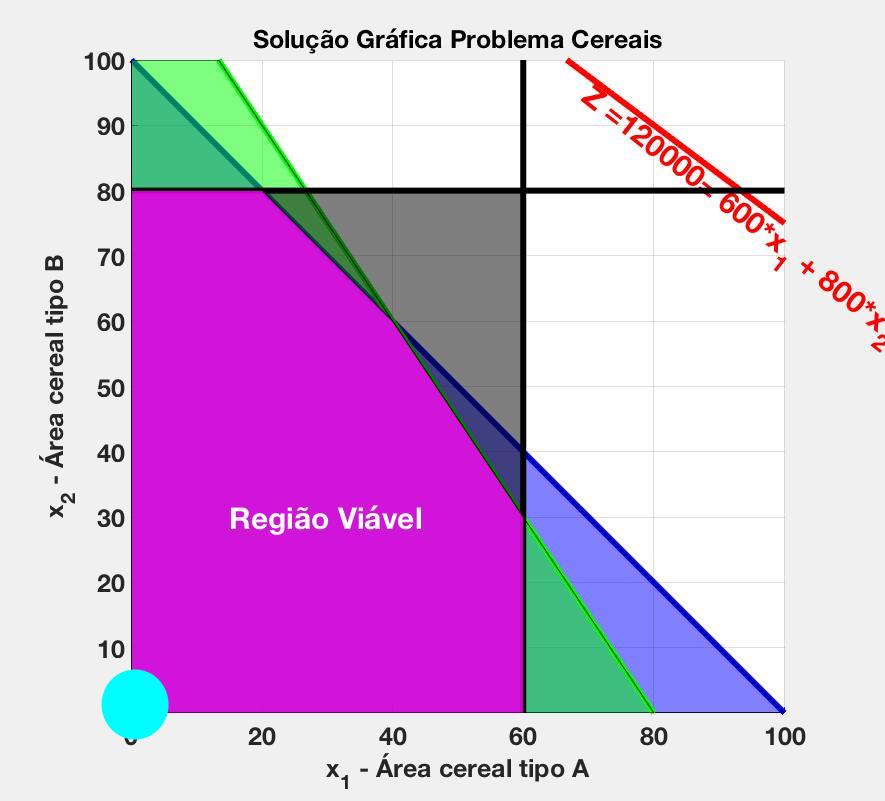
\includegraphics[width=2.8cm,height=2.8cm]{Exaustiva_2.jpeg}
		\end{column}
	\end{columns}
	}
	\only<2>
	{
	\begin{columns}
		\begin{column}{0.5\textwidth}
			\centering
			\begin{mdframed}[backgroundcolor=olive!80]
				Escolhe variável com coeficiente mais negativo na FOB para entrar na base.
			\end{mdframed}
		\end{column}
		\begin{column}{0.5\textwidth}
			\centering
			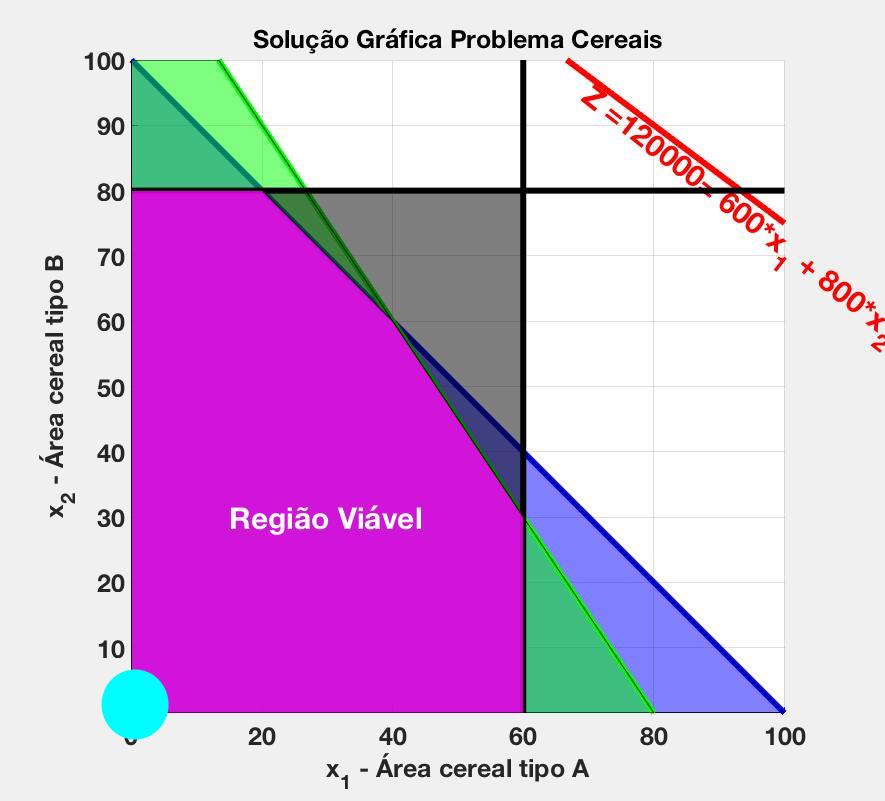
\includegraphics[width=2.8cm,height=2.8cm]{Exaustiva_2.jpeg}
		\end{column}
	\end{columns}	
	}
	\only<3>
	{
	\begin{columns}
		\begin{column}{0.5\textwidth}
			\centering
			\begin{mdframed}[backgroundcolor=orange!80]
				Para cada linha do Tableau calcular razão $\frac{b_i}{\text{coluna}}$. Existe razão positiva e finita?
			\end{mdframed}
		\end{column}
		\begin{column}{0.5\textwidth}
			\centering
			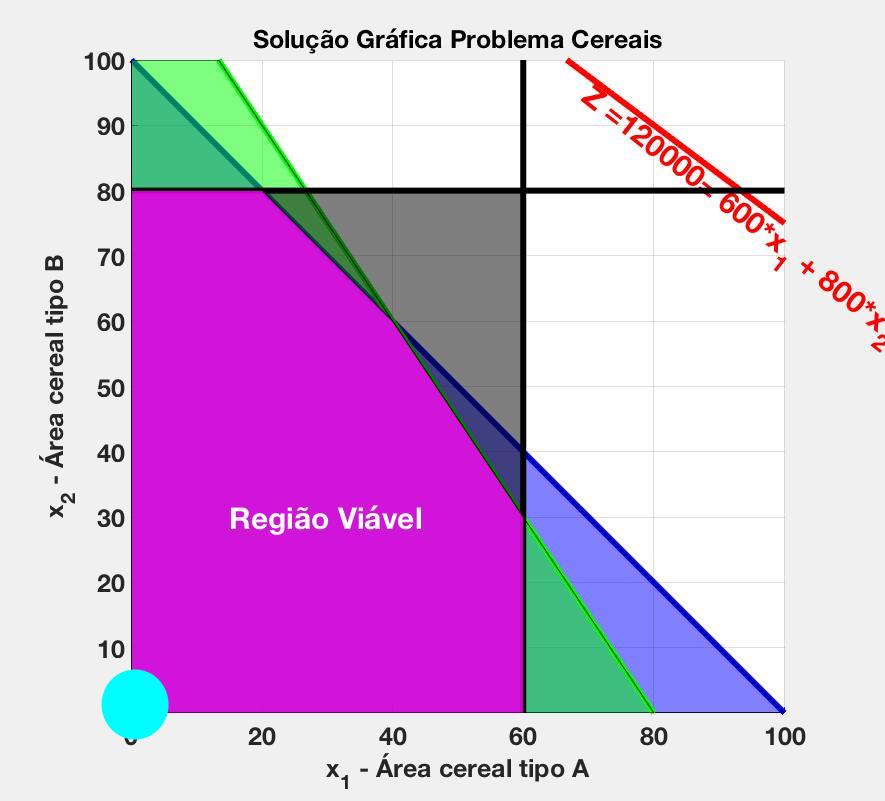
\includegraphics[width=2.8cm,height=2.8cm]{Exaustiva_2.jpeg}
		\end{column}
	\end{columns}	
	}
	\only<4>
	{
	\begin{columns}
		\begin{column}{0.5\textwidth}
			\centering
			\begin{mdframed}[backgroundcolor=olive!80]
				A linha com a menor razão positiva finita sairá da base.
			\end{mdframed}
			$
				\begin{matrix}
					\scriptstyle \text{Linha}'_1 = \text{Linha}_1 - \text{Linha}_4 &  
					\scriptstyle \text{Linha}'_2 = \text{Linha}_2 - 2*\text{Linha}_4 \\  
					\scriptstyle \text{Linha}'_3 = \text{Linha}_3  &  
					\scriptstyle \text{Linha}'_4 = \text{Linha}_4 \\  
					\scriptstyle \text{Linha}'_5 = \text{Linha}_5 + 800*\text{Linha}_4 & \\
				\end{matrix}
			$
		\end{column}
		\begin{column}{0.5\textwidth}
			\centering
			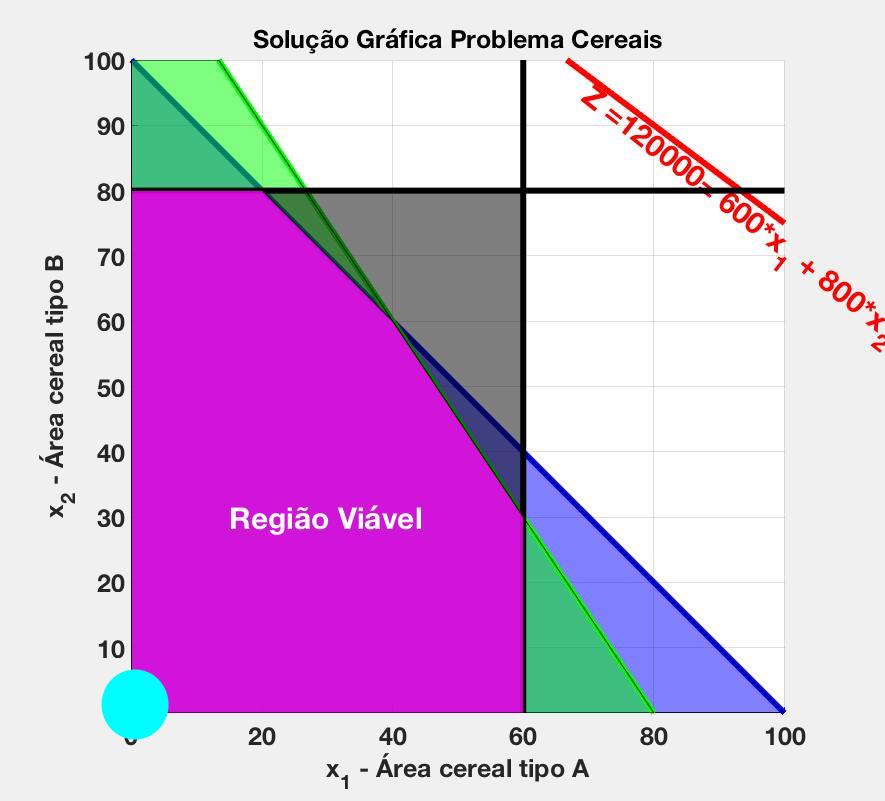
\includegraphics[width=2.8cm,height=2.8cm]{Exaustiva_2.jpeg}
		\end{column}
	\end{columns}	
	}
% % % % % % % % % % % % % % % % % % % % % % % % % % % % % % % % % % % % % % % % % % %
	\only<5>
	{
	\begin{columns}
		\begin{column}{0.5\textwidth}
			\centering
			\begin{mdframed}[backgroundcolor=orange!80]
				Verificar se a solução é ótima! (Linha de Z).
			\end{mdframed}
		\end{column}
		\begin{column}{0.5\textwidth}
			\centering
			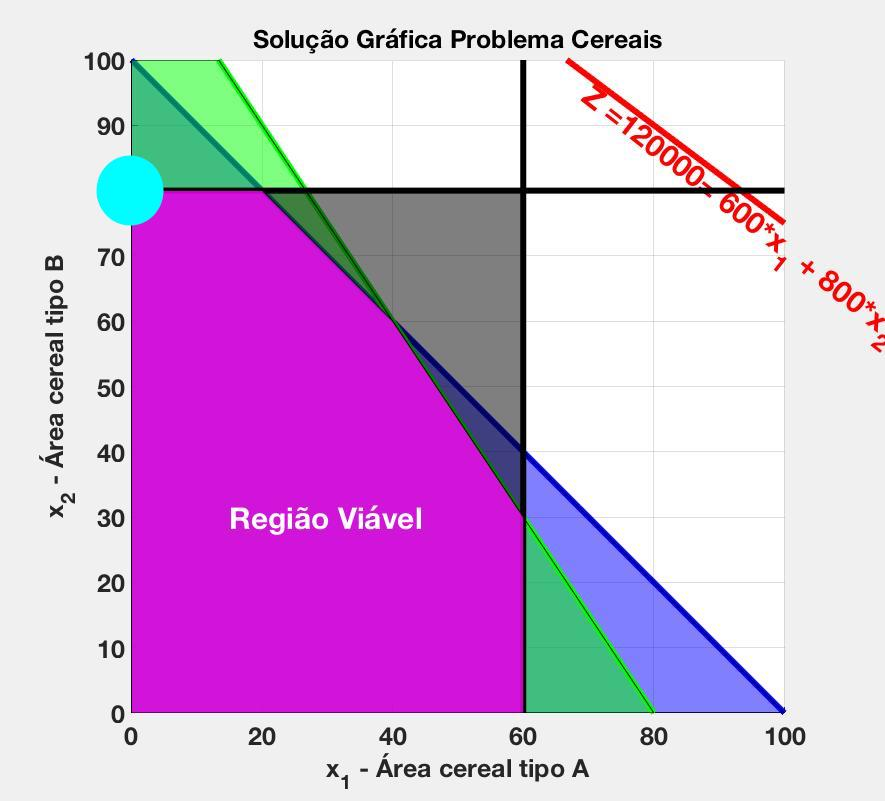
\includegraphics[width=2.8cm,height=2.8cm]{Exaustiva_7.jpeg}
		\end{column}
	\end{columns}
	}
	\only<6>
	{
	\begin{columns}
		\begin{column}{0.5\textwidth}
			\centering
			\begin{mdframed}[backgroundcolor=olive!80]
				Escolhe variável com coeficiente mais negativo na FOB para entrar na base.
			\end{mdframed}
		\end{column}
		\begin{column}{0.5\textwidth}
			\centering
			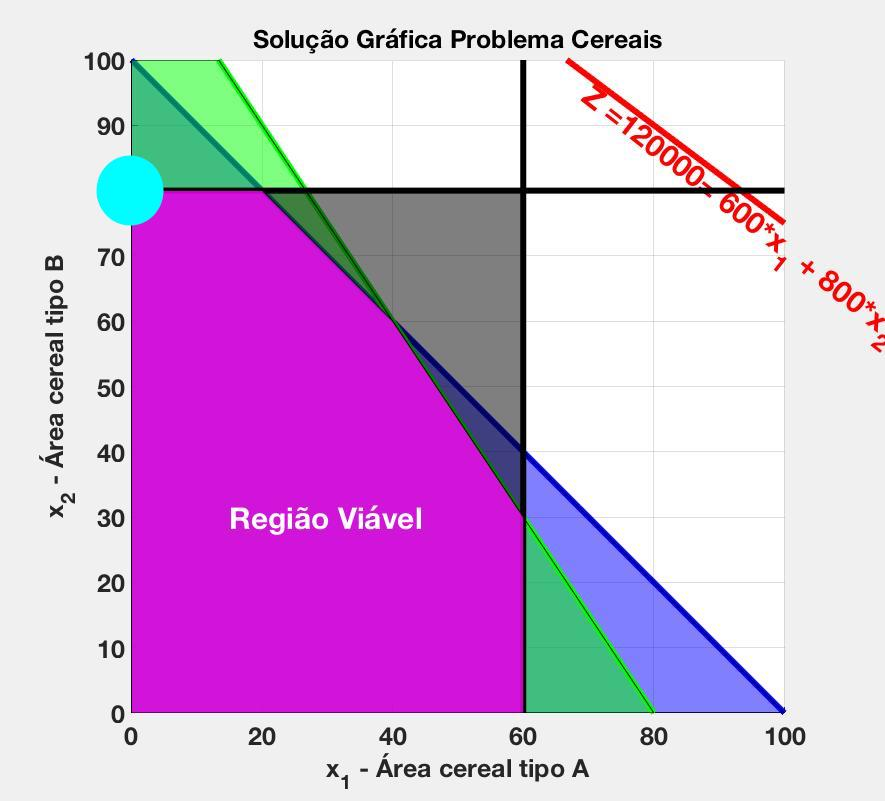
\includegraphics[width=2.8cm,height=2.8cm]{Exaustiva_7.jpeg}
		\end{column}
	\end{columns}	
	}
	\only<7>
	{
	\begin{columns}
		\begin{column}{0.5\textwidth}
			\centering
			\begin{mdframed}[backgroundcolor=orange!80]
				Para cada linha do Tableau calcular razão $\frac{b_i}{\text{coluna}}$. Existe razão positiva e finita?
			\end{mdframed}
		\end{column}
		\begin{column}{0.5\textwidth}
			\centering
			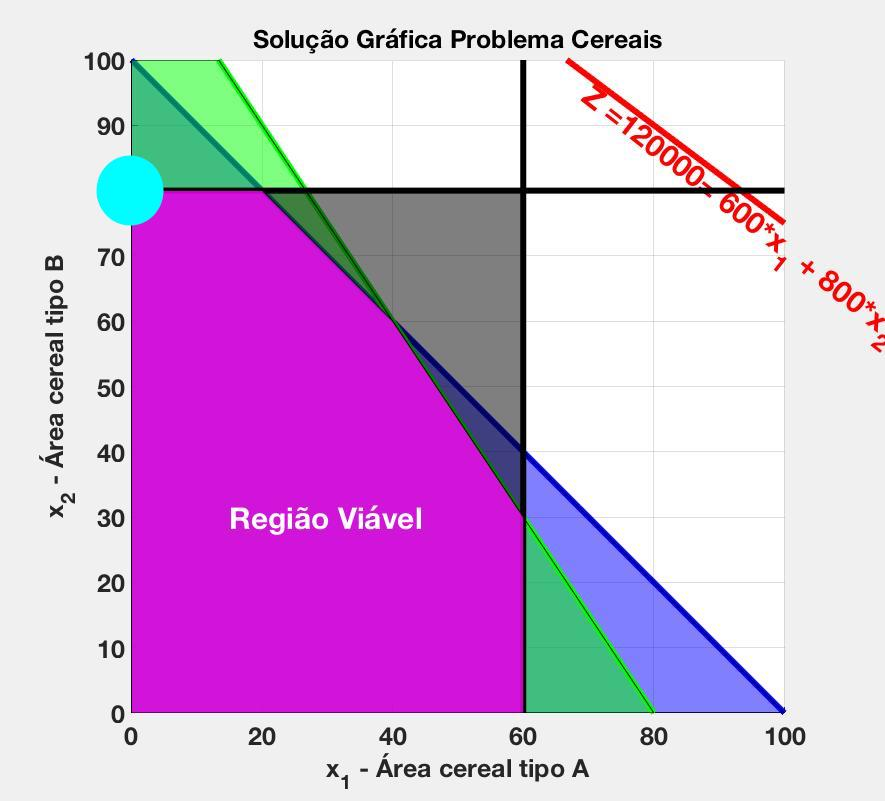
\includegraphics[width=2.8cm,height=2.8cm]{Exaustiva_7.jpeg}
		\end{column}
	\end{columns}	
	}
	\only<8>
	{
	\begin{columns}
		\begin{column}{0.5\textwidth}
			\centering
			\begin{mdframed}[backgroundcolor=olive!80]
				A linha com a menor razão positiva finita sairá da base.
			\end{mdframed}
			$
				\begin{matrix}
					\scriptstyle \text{Linha}'_1 = \text{Linha}_1 &  
					\scriptstyle \text{Linha}'_2 = \text{Linha}_2 - 3*\text{Linha}_1 \\  
					\scriptstyle \text{Linha}'_3 = \text{Linha}_3 - \text{Linha}_1 &  
					\scriptstyle \text{Linha}'_4 = \text{Linha}_4 \\  
					\scriptstyle \text{Linha}'_5 = \text{Linha}_5 + 600*\text{Linha}_1 & \\
				\end{matrix}
			$
		\end{column}
		\begin{column}{0.5\textwidth}
			\centering
			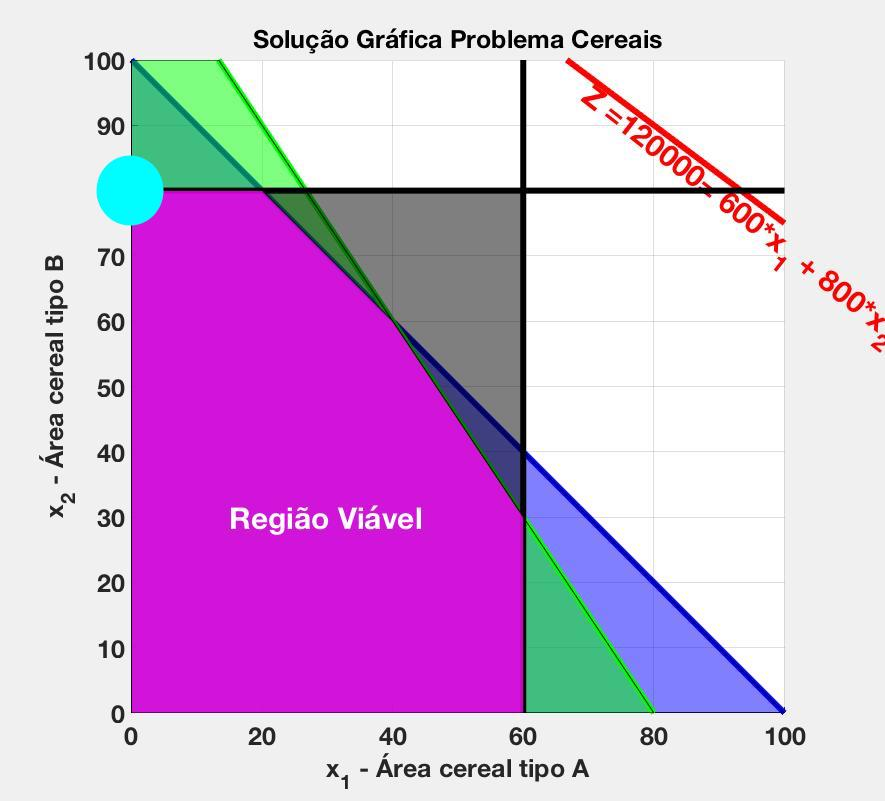
\includegraphics[width=2.8cm,height=2.8cm]{Exaustiva_7.jpeg}
		\end{column}
	\end{columns}	
	}
	% % % % % % % % % % % % % % % % % % % % % % % % % % % % % % % % % % % % % % % % % % % %
	\only<9>
	{
	\begin{columns}
		\begin{column}{0.5\textwidth}
			\centering
			\begin{mdframed}[backgroundcolor=red!80]
				\centering
				OPTIMAL SOLUTION FOUND !!!!
			\end{mdframed}
		\end{column}
		\begin{column}{0.5\textwidth}
			\centering
			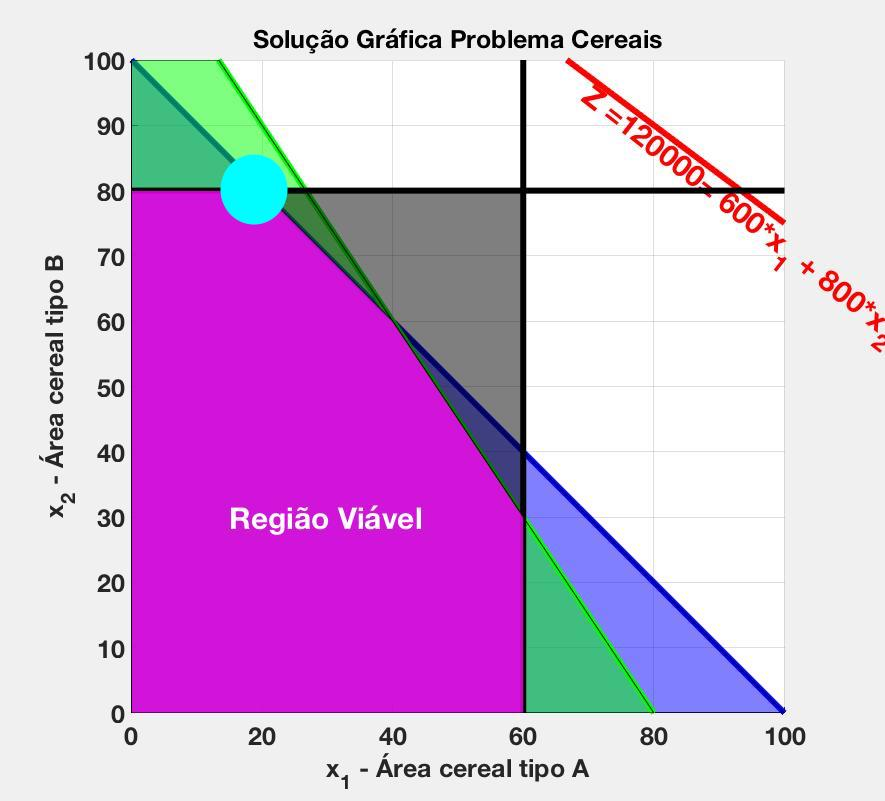
\includegraphics[width=2.8cm,height=2.8cm]{Exaustiva_6.jpeg}
		\end{column}
	\end{columns}
	}	
\end{frame}

\begin{frame}
	\begin{columns}
		\begin{column}{0.5\textwidth}
			\centering
			
\includegraphics[width=4cm,height=4cm]{alegre.jpg}
			\begin{mdframed}[backgroundcolor=cyan!80]
				\centering
				Simplex: 3 Iterações !!!!
			\end{mdframed}
		\end{column}
		\begin{column}{0.5\textwidth}
			\centering
			
\includegraphics[width=4cm,height=4cm]{triste.jpg}
			\begin{mdframed}[backgroundcolor=gray!60]
				\centering
				Exaustão: Análise de 15 Combinações !!!!
			\end{mdframed}
		\end{column}
	\end{columns}
\end{frame}